% NodeDiffusionTransformer vs TextCondGNN — BERT + Cross-Attention architecture
% Compile: xelatex type_classifier_arch.tex
\documentclass[tikz, border=14pt]{standalone}
\usepackage{amsmath}
\usepackage{tikz}
\usetikzlibrary{positioning, arrows.meta, fit, backgrounds, calc}

\definecolor{Ci}{RGB}{207,226,248}   % blue  – inputs / outputs
\definecolor{Ce}{RGB}{250,228,182}   % amber – embedding
\definecolor{Cs}{RGB}{188,220,230}   % steel – encoder
\definecolor{Cp}{RGB}{247,202,202}   % pink  – coord head
\definecolor{Cg}{RGB}{198,232,198}   % green – type head
\definecolor{Ct}{RGB}{220,240,220}   % mint  – BERT branch
\definecolor{Cbdr}{RGB}{148,148,148}

\tikzset{
  Bs/.style n args={1}{draw=Cbdr, fill=#1, rounded corners=3pt,
    minimum width=2.0cm, minimum height=0.68cm,
    align=center, inner sep=4pt, font=\small\sffamily},
  Bm/.style n args={1}{draw=Cbdr, fill=#1, rounded corners=3pt,
    minimum width=2.6cm, minimum height=0.68cm,
    align=center, inner sep=4pt, font=\small\sffamily},
  BnL/.style n args={1}{draw=Cbdr, fill=#1, rounded corners=3pt,
    minimum width=5.2cm, minimum height=0.68cm,
    align=center, inner sep=4pt, font=\small\sffamily},
  BnR/.style n args={1}{draw=Cbdr, fill=#1, rounded corners=3pt,
    minimum width=4.2cm, minimum height=0.68cm,
    align=center, inner sep=4pt, font=\small\sffamily},
  grp/.style={draw=Cbdr!50, fill=black!3, rounded corners=6pt,
    line width=0.7pt, dashed},
  ttl/.style={font=\small\sffamily\bfseries, text=black!65},
  a/.style={-{Stealth[length=5pt,width=4pt]}, line width=0.9pt, color=black!50},
  eq/.style={draw=black!25, dashed, line width=0.6pt}
}

\begin{document}
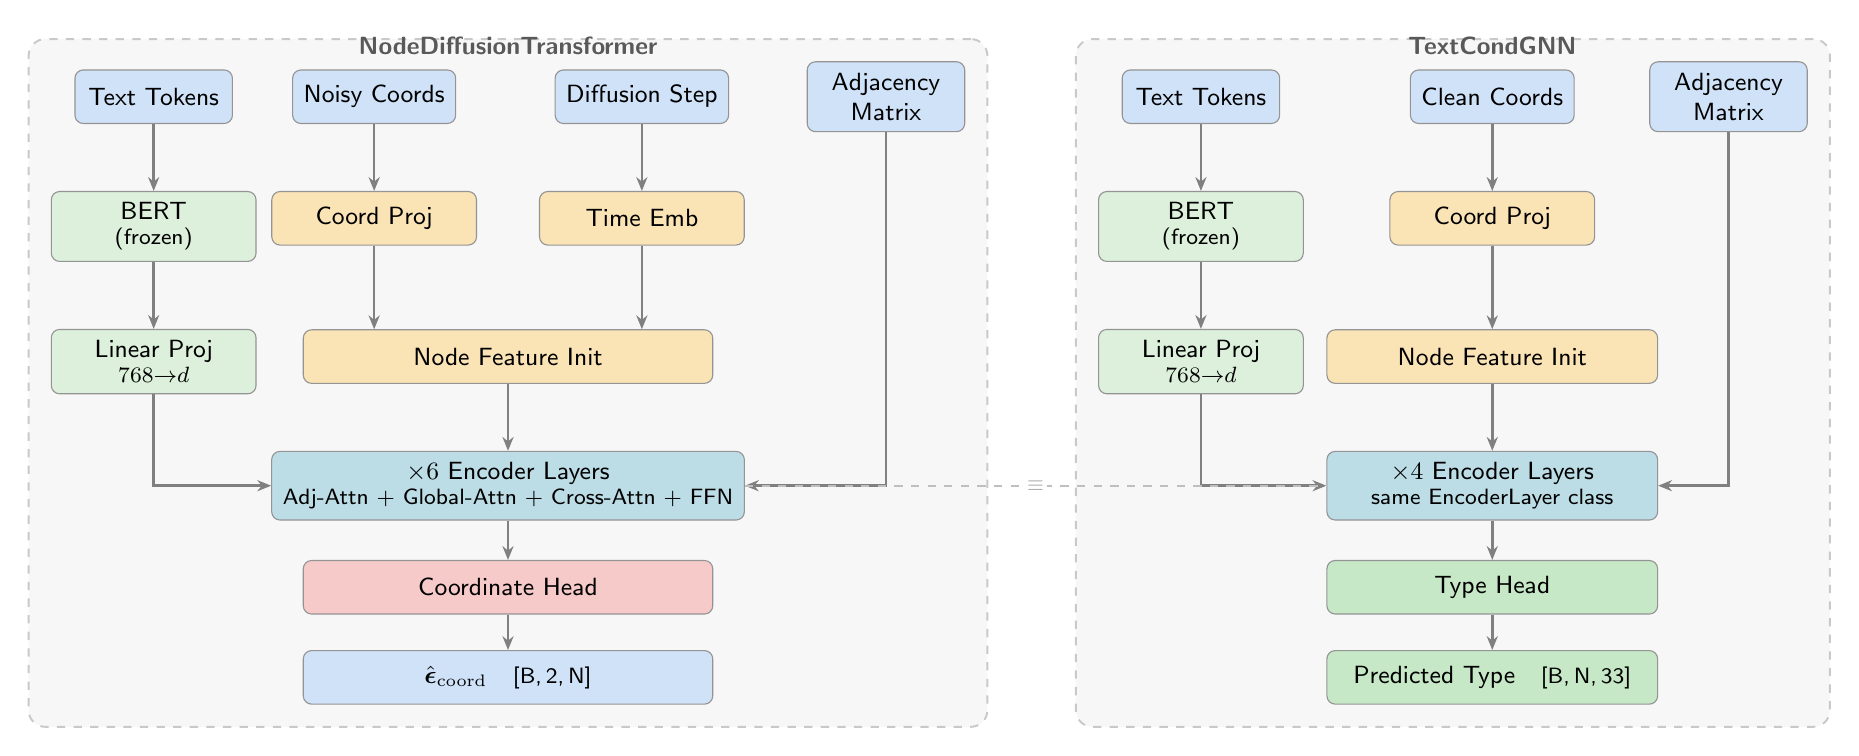
\begin{tikzpicture}

% ═══════════════════════════════════════════════════════════════
%  LEFT  NodeDiffusionTransformer
%  Text branch x=-9.0  |  Coord x=-6.2  Time x=-2.8  |  Adj x=0.3
% ═══════════════════════════════════════════════════════════════
\node[ttl] at (-4.5, 0.65) {NodeDiffusionTransformer};

\node[Bs={Ci}] (Ltxt) at (-9.0,  0) {Text Tokens};
\node[Bs={Ci}] (Lxin) at (-6.2,  0) {Noisy Coords};
\node[Bs={Ci}] (Ltin) at (-2.8,  0) {Diffusion Step};
\node[Bs={Ci}] (Ladj) at ( 0.3,  0) {Adjacency\\Matrix};

\node[Bm={Ct}, below=0.85cm of Ltxt] (Lbert)
  {BERT\\[-2pt]\footnotesize(frozen)};
\node[Bm={Ce}, below=0.85cm of Lxin] (Lcp) {Coord Proj};
\node[Bm={Ce}, below=0.85cm of Ltin] (Ltm) {Time Emb};

\node[Bm={Ct}, below=0.85cm of Lbert] (Ltp)
  {Linear Proj\\[-2pt]\footnotesize$768{\to}d$};
\node[BnL={Ce}] (Lni) at (-4.5, -3.3) {Node Feature Init};

\node[BnL={Cs}, below=0.85cm of Lni] (Lenc)
  {$\times 6$\ Encoder Layers\\[-2pt]%
   \footnotesize Adj-Attn $+$ Global-Attn $+$ Cross-Attn $+$ FFN};

\node[BnL={Cp}, below=0.5cm of Lenc] (Lhd) {Coordinate Head};
\node[BnL={Ci}, below=0.45cm of Lhd] (Lout)
  {$\hat{\boldsymbol{\epsilon}}_{\mathrm{coord}}$\quad\footnotesize[B,\,2,\,N]};

\draw[a] (Ltxt) -- (Lbert);
\draw[a] (Lbert) -- (Ltp);
\draw[a] (Lxin) -- (Lcp);
\draw[a] (Ltin) -- (Ltm);
\draw[a] (Lcp.south) -- (Lcp.south |- Lni.north);
\draw[a] (Ltm.south) -- (Ltm.south |- Lni.north);
\draw[a] (Lni)  -- (Lenc);
\draw[a] (Lenc) -- (Lhd);
\draw[a] (Lhd)  -- (Lout);
\draw[a] (Ltp.south) |- (Lenc.west);
\draw[a] (Ladj.south) -- (Ladj.south |- Lenc.east) -- (Lenc.east);

\begin{scope}[on background layer]
  \node[grp,
        fit=(Ltxt)(Lxin)(Ltin)(Ladj)(Lbert)(Lcp)(Ltm)(Ltp)(Lni)(Lenc)(Lhd)(Lout),
        inner sep=8pt] (Gleft) {};
\end{scope}

% ═══════════════════════════════════════════════════════════════
%  RIGHT  TextCondGNN
%  Text branch x=2.8  |  Coord x=8.0  |  Adj x=10.5
%  Rni/Renc center x=6.5  (clear of Rtp right edge at 4.1)
% ═══════════════════════════════════════════════════════════════
\node[ttl] at (8.0, 0.65) {TextCondGNN};

\node[Bs={Ci}] (Rtxt) at ( 4.3, 0) {Text Tokens};
\node[Bs={Ci}] (Rxin) at ( 8.0, 0) {Clean Coords};
\node[Bs={Ci}] (Radj) at (11.0, 0) {Adjacency\\Matrix};

\node[Bm={Ct}, below=0.85cm of Rtxt] (Rbert)
  {BERT\\[-2pt]\footnotesize(frozen)};
\node[Bm={Ce}, below=0.85cm of Rxin] (Rcp) {Coord Proj};  % x follows Rxin = 6.5

\node[Bm={Ct}, below=0.85cm of Rbert] (Rtp)
  {Linear Proj\\[-2pt]\footnotesize$768{\to}d$};
\node[BnR={Ce}] (Rni) at (8.0, -3.3) {Node Feature Init};

\node[BnR={Cs}, below=0.85cm of Rni] (Renc)
  {$\times 4$\ Encoder Layers\\[-2pt]%
   \footnotesize same EncoderLayer class};

\node[BnR={Cg}, below=0.5cm of Renc] (Rhd) {Type Head};
\node[BnR={Cg}, below=0.45cm of Rhd] (Rout)
  {Predicted Type\quad\footnotesize[B,\,N,\,33]};

\draw[a] (Rtxt) -- (Rbert);
\draw[a] (Rbert) -- (Rtp);
\draw[a] (Rxin) -- (Rcp);
\draw[a] (Rcp.south) -- (Rcp.south |- Rni.north);
\draw[a] (Rni)  -- (Renc);
\draw[a] (Renc) -- (Rhd);
\draw[a] (Rhd)  -- (Rout);
\draw[a] (Rtp.south) |- (Renc.west);
\draw[a] (Radj.south) -- (Radj.south |- Renc.east) -- (Renc.east);

\begin{scope}[on background layer]
  \node[grp,
        fit=(Rtxt)(Rxin)(Radj)(Rbert)(Rcp)(Rtp)(Rni)(Renc)(Rhd)(Rout),
        inner sep=8pt] (Gright) {};
\end{scope}

% ═══════════════════════════════════════════════════════════════
%  ≡ connector — Encoder row only (row 3 has no cross-nodes in gap)
% ═══════════════════════════════════════════════════════════════
\draw[eq] (Lenc.east) -- (Renc.west)
  node[midway, font=\scriptsize\sffamily, text=black!35,
       fill=white, inner sep=1pt] {$\equiv$};

\end{tikzpicture}
\end{document}
